\documentclass[handout]{beamer} 
\usepackage[ngerman]{babel}
\usepackage[utf8]{inputenc}
\usepackage[T1]{fontenc}
\usepackage{amsmath,amssymb}
\usepackage{graphicx}
\usepackage{xcolor}
\usepackage{mathptmx} 
\usepackage{outlines} 
\usepackage{listings}
\usepackage{tikz}

\usepackage{multirow}
\usepackage{booktabs}

\usetheme{ntb}

\title[CleanCode]{Clean Code}
\author{Simon Härdi}
\institute{Institute for Computational Engineering}
\date{xx}

\graphicspath{ {pictures/} }

%% general vector style (bold or with arrow)
\newcommand{\ve}[1]{
    \mathbf{#1}
    %\vec{#1}
}

%% common shortcuts
\providecommand{\argmin}{\operatorname*{argmin}} % operatorname makes _{..} appear centered
\providecommand{\argmax}{\operatorname*{argmax}} % operatorname makes _{..} appear centered
\newcommand{\dd}[1]{\,\mathrm{d}#1} % integration: \int f(x) \dd{x}
\newcommand{\EE}{\mathbb{E}}        % expectation value
\newcommand{\RR}{\mathbb{R}}        % set of real numbers
\newcommand{\CC}{\mathbb{C}}        % set of complex numbers
\newcommand{\NN}{\mathbb{N}}        % set of natural numbers
\newcommand{\OO}{\mathcal{O}}       % big O notation (asymptotic complexity)
\newcommand{\TT}{\mathbb{T}}        % time interval

%% Vectors (lowercase letters)
\renewcommand{\a}{\ve{a}}
\renewcommand{\b}{\ve{b}}
\renewcommand{\c}{\ve{c}}
\renewcommand{\d}{\ve{d}}
\newcommand{\e}{\ve{e}}
\newcommand{\f}{\ve{f}}
\newcommand{\g}{\ve{g}}
\newcommand{\h}{\ve{h}}
\renewcommand{\i}{\ve{i}}
\renewcommand{\j}{\ve{j}}
\renewcommand{\k}{\ve{k}}
\renewcommand{\l}{\ve{l}}
\newcommand{\m}{\ve{m}}
\newcommand{\n}{\ve{n}}
\renewcommand{\o}{\ve{o}}
\newcommand{\p}{\ve{p}}
\newcommand{\q}{\ve{q}}
\renewcommand{\r}{\ve{r}}
\newcommand{\s}{\ve{s}}
\renewcommand{\t}{\ve{t}}
\renewcommand{\u}{\ve{u}}
\renewcommand{\v}{\ve{v}}
\newcommand{\w}{\ve{w}}
\newcommand{\x}{\ve{x}}
\newcommand{\y}{\ve{y}}
\newcommand{\z}{\ve{z}}

%% Matrices (uppercase letters)
\newcommand{\A}{\ve{A}}
\newcommand{\B}{\ve{B}}
\newcommand{\C}{\ve{C}}
\newcommand{\D}{\ve{D}}
\newcommand{\E}{\ve{E}}
\newcommand{\F}{\ve{F}}
\newcommand{\G}{\ve{G}}
\renewcommand{\H}{\ve{H}}
\newcommand{\I}{\ve{I}}
\newcommand{\J}{\ve{J}}
\newcommand{\K}{\ve{K}}
\renewcommand{\L}{\ve{L}}
\newcommand{\M}{\ve{M}}
\newcommand{\N}{\ve{N}}
\renewcommand{\O}{\ve{O}}
\renewcommand{\P}{\ve{P}}
\newcommand{\Q}{\ve{Q}}
\newcommand{\R}{\ve{R}}
\renewcommand{\S}{\ve{S}}
\newcommand{\T}{\ve{T}}
\newcommand{\U}{\ve{U}}
\newcommand{\V}{\ve{V}}
\newcommand{\W}{\ve{W}}
\newcommand{\X}{\ve{X}}
\newcommand{\Y}{\ve{Y}}
\newcommand{\Z}{\ve{Z}}

% \codeemph command
\newcommand{\changefont}[3]{\fontfamily{#1}\fontseries{#2}\fontshape{#3}\selectfont}
\newcommand{\codeemph}[1]{{\changefont{pcr}{m}{n}#1}}

\lstset{ %
  language=C++, % choose the language of the code
  %basicstyle=\small\ttfamily, % the size of the fonts that are used for the code
  basicstyle=\footnotesize, % the size of the fonts that are used for the code
  numbers=none, % where to put the line-numbers
  numberstyle=\small\ttfamily\color[rgb]{0.6,0.6,0.6}, % the size of the fonts that are used for the line-numbers
  stepnumber=1, % the step between two line-numbers. If it's 1 each line
  xleftmargin=4mm,
  % will be numbered
  numbersep=5pt, % how far the line-numbers are from the code
  %backgroundcolor=\color{white}, % choose the background color. You must add \usepackage{color}
  showspaces=false, % show spaces adding particular underscores
  showstringspaces=false, % underline spaces within strings
  showtabs=false, % show tabs within strings adding particular underscores
%  frame=l, % adds a frame around the code
  frame=single,
  tabsize=2, % sets default tabsize to 2 spaces
  breaklines=true, % sets automatic line breaking
  breakatwhitespace=false, % sets if automatic breaks should only happen at whitespace
  % also try caption instead of title
  escapeinside={@}{@}, % if you want to add a comment within your code
  morekeywords={*,...}, % if you want to add more keywords to the set
  keywordstyle=\color[rgb]{0,0,1},
  commentstyle=\color[rgb]{0.133,0.545,0.133}\textit,
  stringstyle=\color[rgb]{0.627,0.126,0.941},
}

%% Code
\usepackage{listings}
\lstset{ %
  language=matlab, % choose the language of the code
  basicstyle=\small\ttfamily, % the size of the fonts that are used for the code
  %numbers=left, % where to put the line-numbers
  %numberstyle=\small\ttfamily\color[rgb]{0.6,0.6,0.6}, % the size of the fonts that are used for the line-numbers
  %stepnumber=1, % the step between two line-numbers. If it's 1 each line
  %xleftmargin=4mm,
  %% will be numbered
  %numbersep=5pt, % how far the line-numbers are from the code
  %backgroundcolor=\color{white}, % choose the background color. You must add \usepackage{color}
  %showspaces=false, % show spaces adding particular underscores
  %showstringspaces=false, % underline spaces within strings
  %showtabs=false, % show tabs within strings adding particular underscores
  frame=off, 
  %%frame=single,
  %tabsize=2, % sets default tabsize to 2 spaces
  breaklines=true, % sets automatic line breaking
  keywordstyle=\color[rgb]{0,0,1},
  commentstyle=\color[rgb]{0.133,0.545,0.133}\textit,
  stringstyle=\color[rgb]{0.627,0.126,0.941},
}



\begin{document}

{
\setbeamertemplate{footline}{} % No footer on first slide
\begin{frame}
\maketitle
\end{frame}
}

\section{Einleitung}

\begin{frame}
\frametitle{Einleitung}
\begin{columns}
    \begin{column}{0.6\textwidth}
        \begin{outline}
            \1 Was ist Clean Code?
            \1[]
            \1 Wieso betrifft das uns?
            \1[] (Wir sind doch Ingenieure, keine
            Informatiker\ldots)
        \end{outline}
    \end{column}
    \begin{column}{0.4\textwidth}
        
\includegraphics[width=\linewidth]{cleanCodeBook.jpg}
    \end{column}
\end{columns}
\end{frame}

\begin{frame}[fragile]
    \frametitle{Einführungsbeispiel}
    Ignaz soll einen Bug in einem Code fixen. Er konnte den Fehler auf folgende
    Funktion zurückführen:
\begin{lstlisting}
...
result = testPoints(xCoords,yCoords);
...
\end{lstlisting}
Leider hatte der Autor keine Zeit für Kommentare, und Ignaz ist nicht sicher,
was die Funktion eigentlich machen soll. Helft Ignaz herauszufinden,
was die Funktion \codeemph{testPoints} tut und wo der Fehler liegt.
\end{frame}

\begin{frame}
    \frametitle{Inhalt}
    \tableofcontents
\end{frame}



\begin{frame}
    \frametitle{Grundsatz:}
    \begin{center}
        \huge \bf Code wird öfters gelesen als geschrieben
    \end{center}
    \vspace{2em}\pause
    Also nicht \textit{'Wie schreibe ich schnell Code?'}, \\
    sondern \textit{'Wie schreibe ich schnell \textbf{zu lesenden} Code?'}
\end{frame}

\begin{frame}
    \frametitle{Wann ist Code einfach zu lesen?}
    \begin{center}
        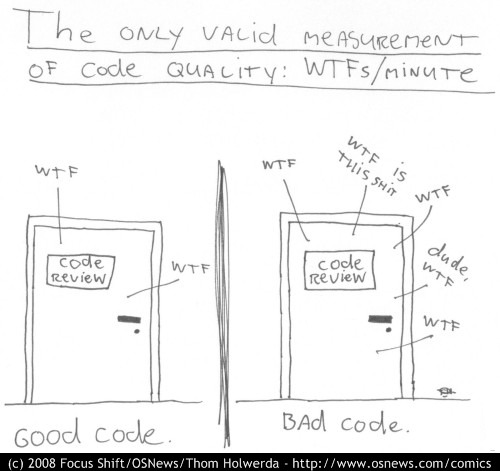
\includegraphics[width=7cm]{wtfm.jpg}
    \end{center}
\end{frame}

\section{Basics}
\begin{frame}
    \tableofcontents[currentsection]
\end{frame}
\subsection{Namen}
\begin{frame}
    \frametitle{Namen}
    \begin{outline}
        \1 Namen sollen Beschreiben
        \1 Lange Namen kein Problem
        \1 Keine Füllwörter
    \end{outline}
\end{frame}

\subsection{Funktionen}
\begin{frame}
    \frametitle{Funktionen}
    \begin{outline}
        \1 Kurz
        \1 Kürzer!
        \1 Nur eine Sache
        \1 Möglichst wenig Argumente
    \end{outline}
\end{frame}

\subsection{Kommentare}
\begin{frame}
    \frametitle{Kommentare}
    \begin{outline}
        \1 Kommentare sind \emph{nicht} per se gut
        \1 Auskommentierter Code
        \1 Nicht mehr aktuelle Kommentare
    \end{outline}
\end{frame}

\section{Erweitert}
\subsection{Tests}
\begin{frame}
    \frametitle{Tests}
    \begin{outline}
        \1 Jeder schreibt Tests 
        \1[] $\Rightarrow$  Wieso nur in Konsole?
        \1 Gehören zum Code dazu
        \1 Alles Testen
            \2 Jede Funktion
            \2 Möglichst jeden Spezialfall
    \end{outline}
\end{frame}
\subsection{Test Driven Development}
\begin{frame}
    \frametitle{Test Driven Development}
    \begin{outline}
        \1 Tests \emph{vor} der Funktion schreiben
        \1 Ein Test $\rightarrow$ Eine Funktion $\rightarrow$ repeat
    \end{outline}
\end{frame}
\subsection{Successive Refinement}
\begin{frame}
    \frametitle{Successive Refinement}
    \begin{outline}
        \1 Code ist \emph{nicht} fertig, sobald er funktioniert
        \1 Kontinuierlich verbessern
        \1 Dank Tests keine Angst, etwas kaputt zu machen
    \end{outline}
\end{frame}

\section{Fazit}
\begin{frame}
    \frametitle{Fazit}
    \begin{outline}
        \1 Beschreibende Namen
        \1 Kurze Funktionen
        \1 Kommentare überlegt benutzen
        \1 Versionierungssystem benutzen
        \1 Tests \emph{zuerst} schreiben
    \end{outline}
\end{frame}

\end{document}
